\phantomsection\numberedsection{RF2.4 Borrar Producto}

\subsection*{Descripción}
Los usuarios deben de poder borrar cualquier producto creado.\par
\vspace{0.15cm}

\textbf{Pre-condición}\par
El usuario debe haber iniciado sesión en su cuenta en Mini PIM y haber creado al menos un producto.\par
\vspace{0.15cm}

\textbf{Post-condición}
\begin{itemize}
    \item Caso de éxito: Se ha borrado exitosamente el producto.
    \item Caso mínimo: El sistema notifica al usuario el resultado de la accion borrar producto; exitosa o fallida.
\end{itemize}

\textbf{Prioridad: }
Alta
\vspace{0.15cm}

\textbf{Autor: }
Angel Nicolas Escaño Lopez y Diego Sicre\par
\vspace{0.15cm}

\textbf{Control de cambios: } Versión 1: Definición del caso de uso

\numberedsubsection{Escenario principal}
\begin{enumerate}
    \item El usuario se encuentra en el apartado de productos y selecciona la opción de \enquote{Borrar}, que es una imagen con una papelera justo después de dicho producto.
    \item El sistema muestra un menú con un botón de confirmar.
    \item El usuario confirma el borrado.
    \item El sistema muestra la página de productos sin el producto borrado.
\end{enumerate}

\numberedsubsection{Escenarios alternativos}
\begin{description}
    \item[2.a.] El usuario cancela la acción de borrar un producto seleccionando la opción que cierra el menú de creación.
    \begin{enumerate}
        \item[2.a.1] El sistema regresa al usuario al apartado de visualización de productos sin modificar nada.
    \end{enumerate}
\end{description}

\numberedsubsection{Casos de Prueba}
\underline{Escenario: Principal}\par
\vspace{0.15cm}
\textbf{Dado} que hay al menos un producto creado,\par
\textbf{Y} estoy en el apartado de Productos,\par
\textbf{Cuando} selecciono la opción de \enquote{Borrar},\par
\textbf{Y} Selecciono \enquote{Confirmar},\par
\textbf{Entonces} el sistema borra la información de la base de datos de Mini PIM,\par
\textbf{Y} actualiza la información del total de productos registrados en la base de datos,\par
\textbf{Y} muestra el apartado de visualización de productos sin el producto borrado.\par
\vspace{0.20cm}

\underline{Escenario: Alternativo 2.a}\par
\vspace{0.15cm}
\textbf{Dado} que hay un producto creado,\par
\textbf{Y} estoy en el apartado de visualización de productos,\par
\textbf{Cuando} selecciono la opción de \enquote{Borrar},\par
\textbf{Y} selecciono la opción de cancelar,\par
\textbf{Entonces} el sistema muestra el apartado de visualización de productos mostrando todos los recursos almacenados sin ningún cambio.\par
\vspace{0.20cm}

\numberedsubsection{Bocetos}
\begin{figure}[H]
    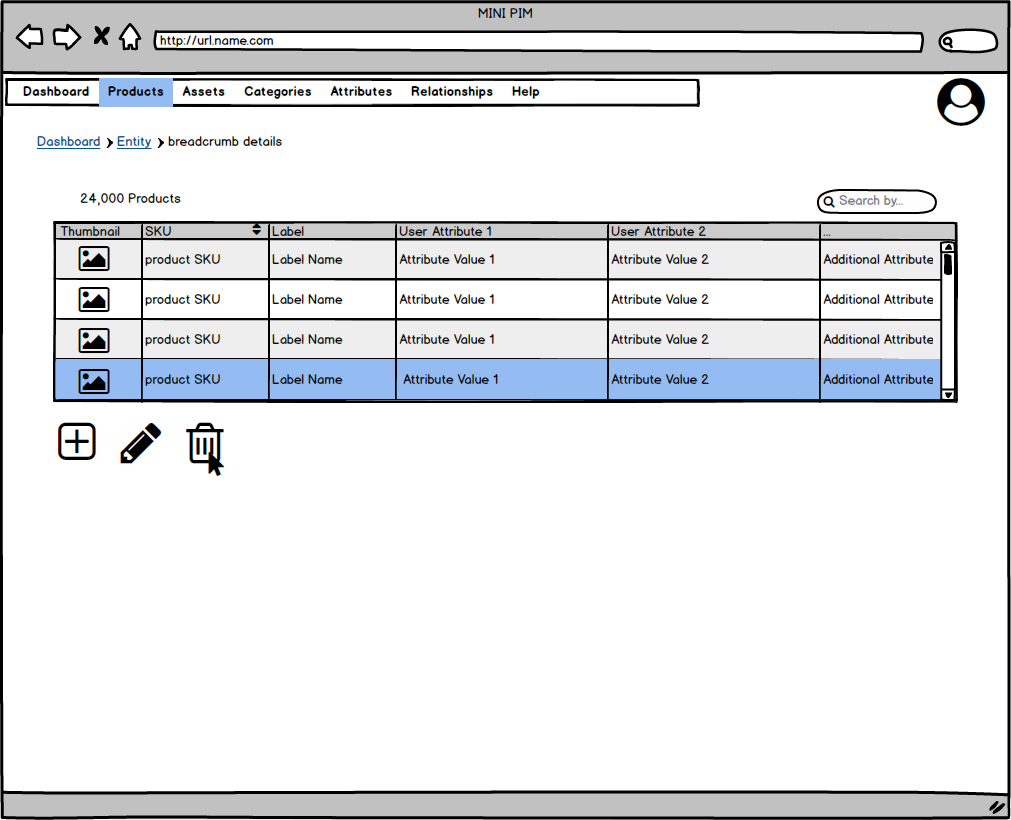
\includegraphics[width=1\linewidth]{mockups/RF2-X Borrar Producto (Borrar Producto desde listado).png}
    \caption{Apartado Productos hacer clic en \enquote{Borrar}}
   \end{figure}
\vspace{1.0cm}

\begin{figure}[H]
    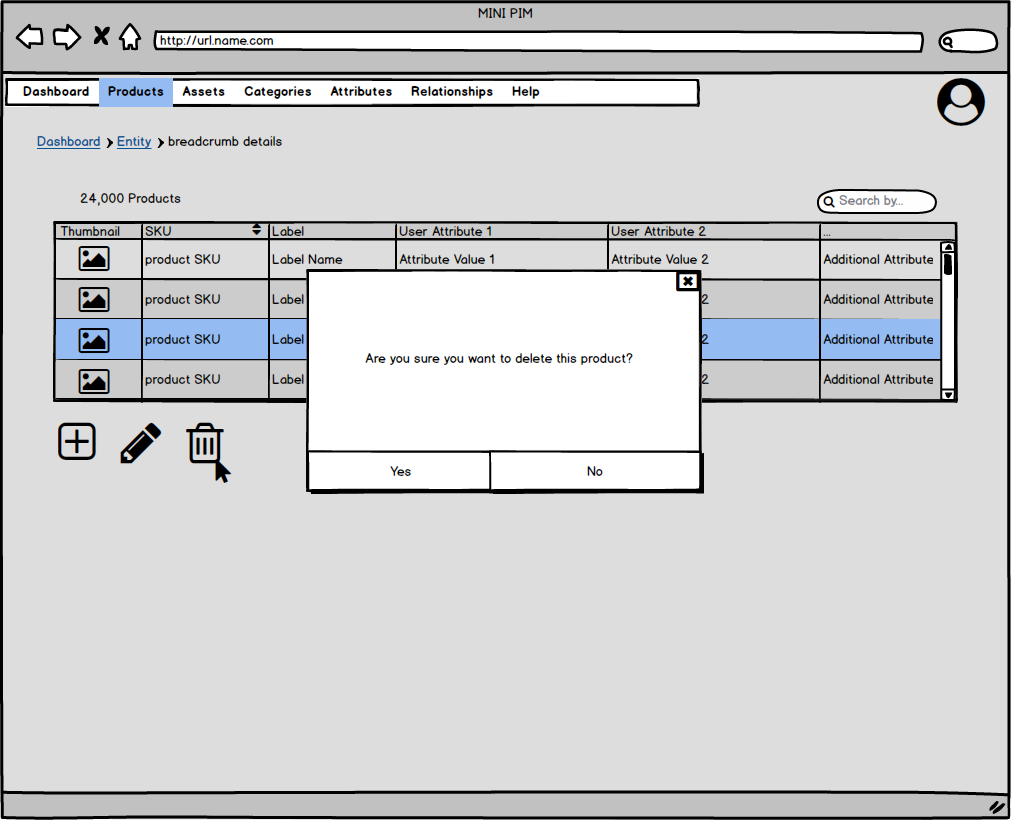
\includegraphics[width=1\linewidth]{mockups/RF2-X Borrar Producto (Borrar Producto Paso1)V2.png}
    \caption{Apartado Productos tras clicar \enquote{Borrar}}
   \end{figure}
\vspace{1.0cm}

\begin{figure}[H]
    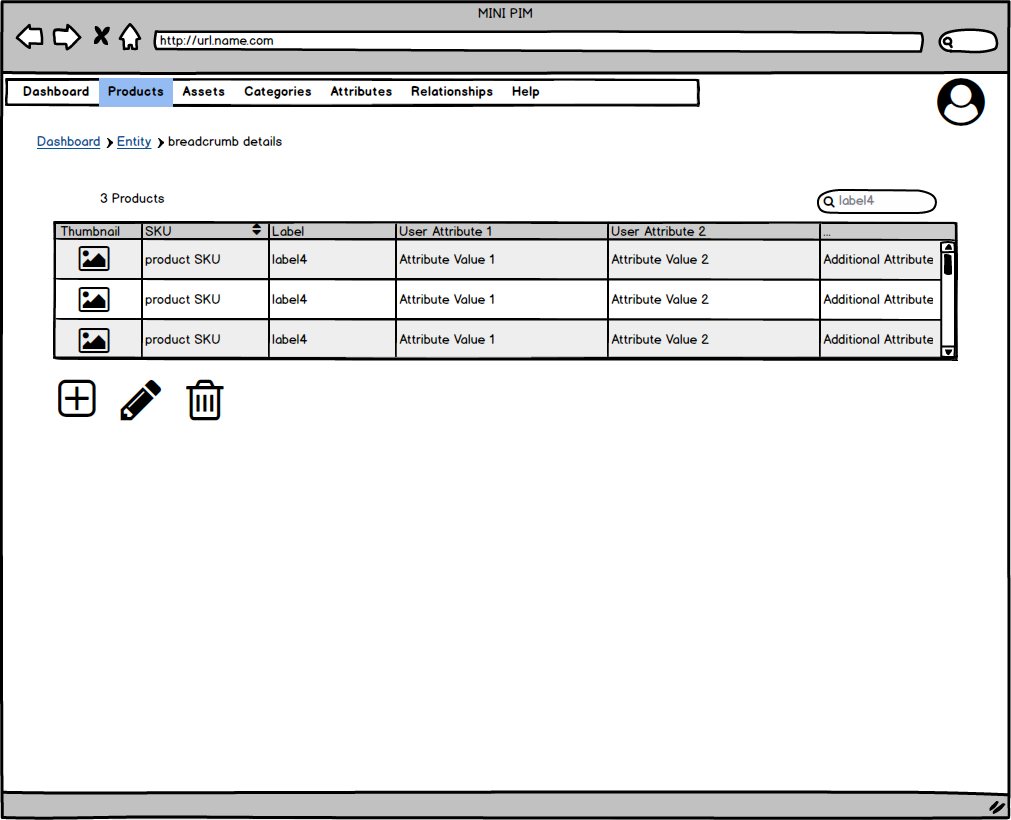
\includegraphics[width=1\linewidth]{mockups/RF2-X Borrar Producto (Borrar Producto Paso2).png}
    \caption{Apartado Productos tras producto borrado}
   \end{figure}
\vspace{1.0cm}

\newpage %Inicia en una nueva página otro caso de uso